\documentclass[../ECON-281-Notes.tex]{subfiles}
\begin{document}
\chapter{Cost and Cost Minimization}
In this chapter we will talk about 
\begin{itemize}
    \item Explicit and implicit cost and sunk cost
    \item Difference between economic and accounting profit
    \item Iso-Cost Line 
    \item Cost minimization problem 
    \item Derivation of the demand curve for labor
    \item Price elasticity of demand for input 
\end{itemize}
\section{Cost Concepts for Decision Making}

\begin{Definition}
    {Explicit Costs}
    Involves monetary payments, i.e., you actually pay for this cost
\end{Definition}

\begin{Definition}
    {Implicit Costs}
    Does not involve monetary payment. This is also called opportunity cost. 
\end{Definition}

\begin{Definition}
    {Accounting Cost}
    These are explicit cost
\end{Definition}

\begin{Definition}
    {Economic Cost}
    These are the sum of Implicit and Explicit Costs.

    Meaning Economic Costs are greater than Accounting Costs, and economic profit is less than accounting profits. 
\end{Definition}

\begin{Definition}
    {Sunk Cost}
    These are costs that once, happen, it cannot be recovered. Since the it cannot be recovered we should ignore it and don't let it affect your decision.
\end{Definition}
\newpage
\section{The Cost-Minimization Problem}
\begin{Definition}
    {Iso-Cost Line}
    Shows teh different bundles of \(L\) and \(K\) that has the same total cost \(TC\).

    The equation of the \textbf{Iso-Cost Line} is similar to the budget line
    \begin{equation}
        TC = w\cdot L + r\cdot K    
    \end{equation}

    The slope of the Iso-Cost line is determine like so
    \begin{equation}
        \text{Slope of Iso Cost} = \frac{-w}{r} 
    \end{equation}
    Where:
    \(w\) is the wage rate for the price of labour and \(r\) is the interest rate for the price of capital.

\end{Definition}

\begin{figure}[h]
    \centering
    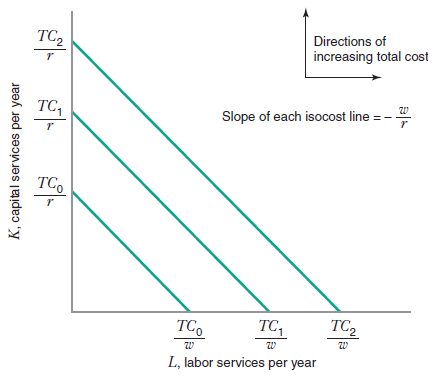
\includegraphics[width=\columnwidth]{../assets/isocost-line.png}
    \caption{Iso-Cost Line}
    \label{fig:iso_cost_line}
\end{figure}


\begin{DndSidebar}[color=PhbLightGreen]{Cost Minization Problem}
    The objective of the producer is to minimize his total cost which will maximize this profits, the goal of every business owner. 

    This is done by finding the best bundle of \(L\) and \(K\) that produces the goods at the lowest cost.

    This is similar to the \emph{Utility Maximization Problem} except instead of maximizing a value we are minimizing a value, in this case it's cost.
\end{DndSidebar}

The cost is minimized when the iso-cost is tangent to the iso-quant. 
\[
    \frac{-w}{r} = MRTS_{LK} = \frac{-MP_L}{MP_K}
\]
Rearranging this equation gives us this
\[
    \frac{MP_L}{w} = \frac{MP_K}{r}
\]
This means cost is minimized when the marginal productivity of a dollar spent on labour equals the marginal productivity of a dollar spent on capital. 

The method of which is similar to finding the maximum utility of a bundle of two goods. 

\begin{figure}[h]
    \centering
    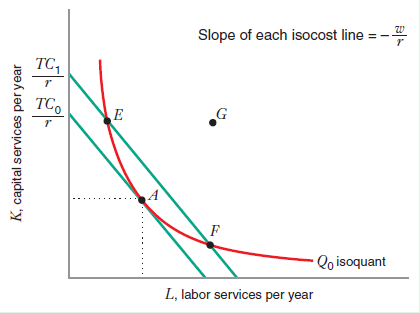
\includegraphics[width=\columnwidth]{../assets/cost-minimizing-input.png}
    \caption{Cost-Minimizing Input Combination}
    \label{fig:cost_min_input}
\end{figure}
In \cref{fig:cost_min_input} Point A is the interior solution for the minimizing the cost.

You can also get a corner solution as well 
\begin{figure}[h]
    \centering
    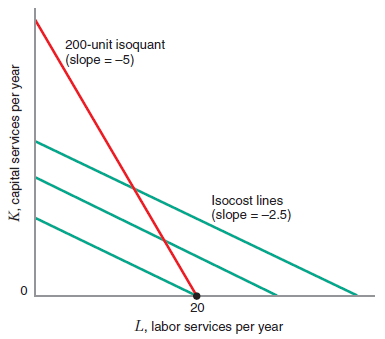
\includegraphics[width=0.9\columnwidth]{../assets/corner-soln-isocost.png}
    \caption{Cost-Minimizing Corner Solution}
    \label{fig:cost_min_corner}
\end{figure}

\section{Comparative Statics Analysis of the Cost-Minimization Problem}
The line that connects const minimizing input bundles due to change in quantity while input prices are constant is called the \textbf{expansion path}.
\begin{figure}[h]
    \centering
    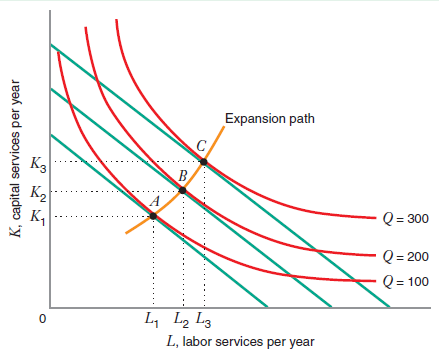
\includegraphics[width=0.9\columnwidth]{../assets/expansion-path-pos.png}   
    \caption{Normal Inputs}
    \label{fig:normal_inputs}
\end{figure}
In \cref{fig:normal_inputs} both inputs are normal therefore an increase in quantity will increase the input for labour and capital.

\begin{figure}[!h]
    \centering
    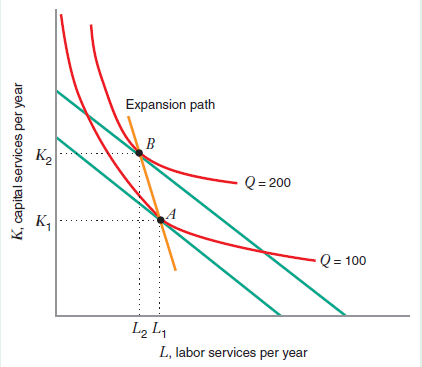
\includegraphics[width=0.9\columnwidth]{../assets/expansion-path-neg.png}   
    \caption{Inferior Inputs}
    \label{fig:inferior_inputs}
\end{figure}
In \cref{fig:inferior_inputs} labour is inferior while capital is normal therefore, an increase in quantity will lead to a decrease in labour and an increase in capital for inputs. 
\newpage
\subsection{Labour Demand Curve}
There is a negative correlation between the cost of labour and the input of labour in production.

\begin{figure}[!h]
    \centering
    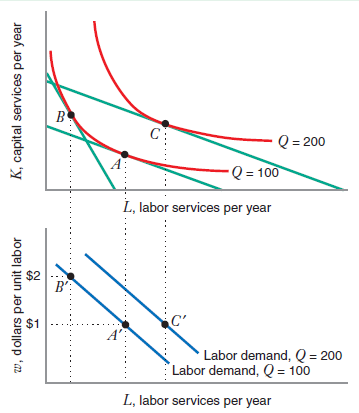
\includegraphics[width=\columnwidth]{../assets/labour_demand_curve.png}   
    \caption{Labour Demand Curve}
    \label{fig:labour_demand_curve}
\end{figure}

\subsection{Price Elasticity of Demand for Inputs}
Like consumption demand there is an elasticity for the demand of input 
\begin{itemize}
    \item \(\varepsilon_{L,w}\) for the price elasticity for labour, or it measures how sensitive \(Q\) of \(L\) to the change in \(w\), other factors kept constant.
    \item \(\varepsilon_{K,r}\) for the price elasticity for capital, or it measures how sensitive \(Q\) of \(K\) to the change in \(r\), other factors kept constant.
\end{itemize}
These elasticity equations follows the same structure as the price elasticity for demand or supply, just replace Quantity \(Q\) with \(L\) or \(K\), and \(P\) with \(w\) or \(r\). This rule works with both the point and arc average formulas. 


\end{document}